\documentclass[a4paper,titlepage]{article}
\usepackage[utf8]{inputenc} %Make sure all UTF8 characters work in the document
\usepackage{listings} %Add code sections
\usepackage{color}
\usepackage{graphicx}
\usepackage{titling}
\usepackage{textcomp}
\usepackage[hyphens]{url}
\usepackage[bottom]{footmisc}
\usepackage[yyyymmdd]{datetime}
\definecolor{listinggray}{gray}{0.9}
\definecolor{lbcolor}{rgb}{0.9,0.9,0.9}
\lstset{	%ifall du ska koda.
		backgroundcolor=\color{lbcolor},
		tabsize=4,
		rulecolor=,
		upquote=true,
		aboveskip={1.5\baselineskip},
		columns=fixed,
		showstringspaces=false,
		extendedchars=true,
	    breaklines=true,
	    prebreak = \raisebox{0ex}[0ex][0ex]{\ensuremath{\hookleftarrow}},
	    frame=single,
	    showtabs=false,
	    showspaces=false,
	    showstringspaces=false,
	    identifierstyle=\ttfamily,
	    keywordstyle=\color[rgb]{0,0,1},
	    commentstyle=\color[rgb]{0.133,0.545,0.133},
	    stringstyle=\color[rgb]{0.627,0.126,0.941},
}

%Set page size
\usepackage{geometry}
\geometry{margin=3cm}
\usepackage{parskip} 

\renewcommand{\dateseparator}{-}
\renewcommand*\contentsname{Innehållsförteckning}
\renewcommand*\figurename{Figur}

\title{
\textbf{Designskiss - The Gentoo Saga} \\
\large TSEA83 Grupp 33}
    \date{\today}
\author{
        Emil Segerbäck - emise935 - emise935@student.liu.se\\
		Malcolm Vigren - malvi108 - malvi108@student.liu.se \\
		Robin Sliwa - robsl733 - robsl733@student.liu.se}
\begin{document}
    \maketitle
    \newpage
\tableofcontents
    \newpage

\section{Inledning}
Vi ska göra en dator som kör spelet The Gentoo Saga. Användaren spelar på ett
tangentbord som kommunicerar med datorn via PS/2 och spelet visas på en
VGA-skärm via dedikerad grafik-hårdvara. Denna hårdvara består av en
grafikmotor, tileminne och spriteminne. Datorn ska också spela musik och
eventuellt ljudeffekter (om vi har tid) via dedikerad ljudhårdvara.

Processorn är av pipeline-typ, liknande till den som användes i
Pipeline-labben, vilket innebär separata program- och dataminnen. 

\section{Spelet}
Spelet går ut på att spelaren ska styra en pingvin som ska försöka nå fram till
en Gentoo-logga i slutet av banan, utan att springa på arga monster eller ramla
av banan på vägen dit. Pingvinen styrs med hjälp av piltangenter där upp används
för att hoppa, och höger och vänster är till för att gå till höger respektive
vänster på skärmen. Banan som pingvinen går på har hål i marken som spelaren kan
ramla igenom. Om man hoppar ovanpå ett monster försvinner det. Om pingvinen
nuddar ett monster från sidan eller ramlar ut ur banan så tar spelet slut. Om
man däremot lyckas ta sig till Gentoo-loggan så klarar man banan.

\section{Analys av problemet}
\begin{itemize}
	\item \textbf{Inmatning}: Modulen som läser in data från tangentbordet
		skriver till ett speciellt register i CPU:n.
	\item \textbf{VGA (bildvisning)}: Vi ska ha en bild på 320x240px vilket
		resulterar i att en storpixel är 4 (2x2) småpixlar. Genom att göra
		detta kommer vi att ha mer tid att rita ut varje pixel på skärmen. 
	\item \textbf{Musik}: Vi ska ha hårdvara som läser musik från speciellt
		musikminne. Den stegar genom noterna som ligger i minnet och spelar upp
		dem i högtalaren.
    \item \textbf{Minne}: Alla register är 32 bitar breda. Vi använder ett 
        programminne, dataminne, tileminne, ett extra tileminne för bakgrund,
        spriteminne och musikminne. Tileminnet har 15x150 tiles. Vi har 32
        olika tiles så tileminnet behöver 15x150x5=11250 bitar=1407 bytes. Det
        andra tileminnet behöver 15x75x4=4500 bitar=563 bytes. Spriteminne
        behöver bara innehålla två sprites på 16x16 pixlar. Musikminne behöver
        instruktioner som har 5 bitar för tonhöjd och 2 bitar för tonlängd,
        totalt 8x128=1024 bitar=128 bytes. Programminnet behöver 2000 
        instruktioner totalt 32x2048=8192 bytes. Till dataminnet tar vi 2048
        bytes. FPGA kortet har 32 blockram, 2kB styck, vilket är mycket mer än
        vår uppskattning. Därför tror vi att minnet kommer att räcka.

\end{itemize}
\newpage
\section{Blockscheman}
    Musikenheten kommer till en början inte att kommunicera med CPUn, kan ses i
    Figur \ref{overviewscheme}, men som ett bör krav har vi ljudeffekter. Detta 
    innebär att om vi senare hinner lägga till ljud effekter så kommer
    musikenheten behöva kommunicera med CPUn.
\begin{figure}[h!]\label{overviewscheme}
	\centering
	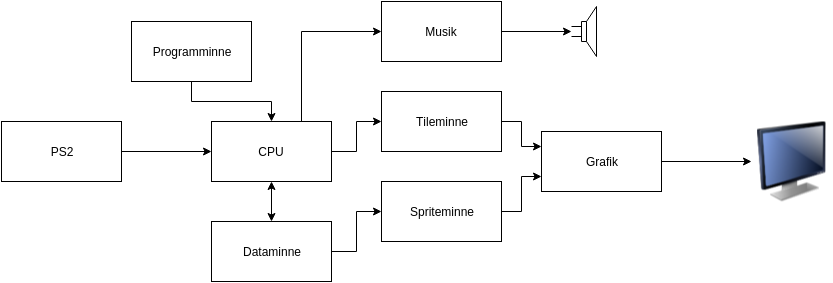
\includegraphics[width=14cm]{overview.png}
	\caption{Översiktligt blockschema}
\end{figure}

Musikmodulen loopar igenom ett speciellt musikminne. Varje element i listan
innehåller tonlängd och -höjd. I modulen har man en räknare som räknar ner tiden
för den nuvarande tonen och en annan modul som bara tar in 5 bitar (32 toner
~2,5 oktaver) som säger vilken ton som ska spelas just nu. De 5 bitarna används
för att slå upp i en tabell över hur långa pulserna ska vara för den tonen. Sen
växlar den bara mellan att skicka ut 0 och 1 på högtalaren.

\begin{figure}[h!]
	\centering
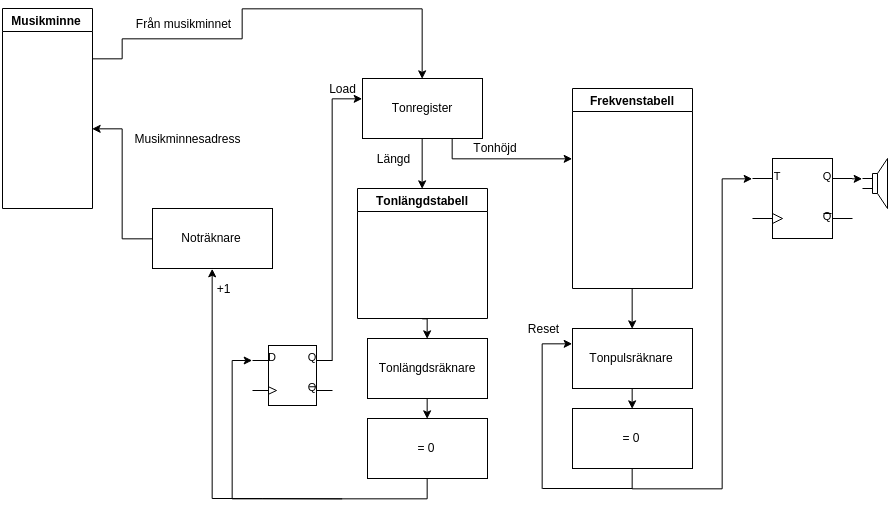
\includegraphics[width=14cm]{Musik.png}
	\caption{Blockschema över musikenheten}
\end{figure}

\begin{figure}[h!]
	\centering
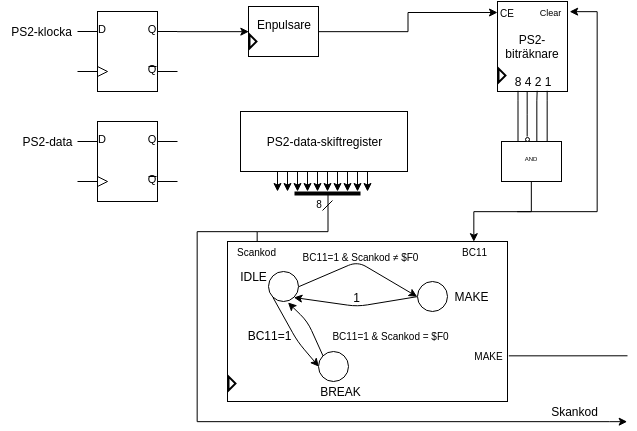
\includegraphics[width=14cm]{PS2.png}
	\caption{Blockschema över PS2-enheten}
\end{figure}

\begin{figure}[h!]
	\centering
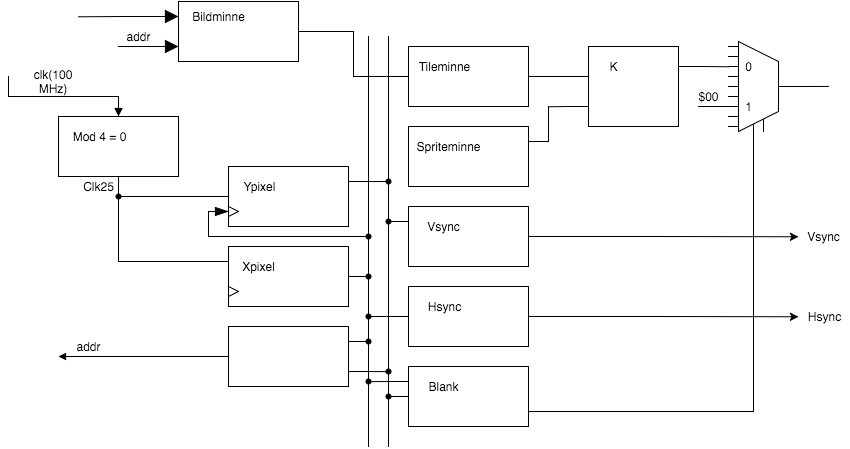
\includegraphics[width=14cm]{vga-schema.png}
	\caption{Blockschema över grafikenheten}
\end{figure}

\section{Milstolpe}
Efter halva projektet ska processorn kunna exekvera alla instruktioner och
grafiken ska kunna rita ut tiles på VGA-skärmen. Detta innebär att tileminnet
är klart och fullt fungerande.
% 
%\newpage
%\section{Checklista}
%    \subsection{Spelimplementation}
%        \begin{itemize}
%            \item Se bild på discord
%            \item Bland annat att PS2-kontrollern skriver till ett register om
%                vilka knappar som är nedtryckta, och endast de som används i
%                spelet. Vi har också spriteminnen.
%        \end{itemize}
%    \subsection{CPU}
%        \begin{itemize}
%            \item Pipeline
%            \item Separata program/dataminnen
%            \item De flesta, om inte alla, instruktioner från lab 2 plus några
%				fler.
%            \item Processorn ska arbeta med 32-bitars ord.
%            \item Eftersom vi använder pipeline är addresseringsmoder inte applicerbart.
%            \item Specialinstruktioner för tiles, sprites och musik.
%            \item Program- och dataminnet ska programmeras via UART.
%            \item Vi ska använda ett separat hårdvarublock för detta.
%            \item Processorn sköter all spelmekanik - AI,
%				kollisionsdetektering, rörelseberäkning etc.
%        \end{itemize}
%	\subsection{Grafik}
%        \begin{itemize}
%			\item Grafiken ritas ut av en separat hårvarukomponent m.h.a. tile-
%				och spriteminne.
%			\item 320x240, 8-bitars färg. Tiles och sprites á 16x16 pixlar.
%			\item CPUn skriver skiten i bildminnet och sedan ritar
%				grafikenheten ut grejerna, så ingen synkronisering behövs.
%        \end{itemize}
%	\subsection{I/O-enheter}
%        \begin{itemize}
%			\item Tangentbord, högtalare och skärm.
%			\item Tangentbordet skriver till ett register i CPUn.
%        \end{itemize}
%	\subsection{Minnesanvändning}
%        \begin{itemize}
%			\item Alla register är 32 bitar breda. Vi använder ett
%				programminne, dataminne, tileminne, ett extra tileminne för
%				bakgrund, spriteminne och musikminne.
%			\item Tileminnet har 15x150 tiles. Vi har 32 olika tiles så
%				tileminnet behöver 15x150x5=11250 bitar=1407 bytes. Det andra
%				tileminnet behöver 15x75x4=4500 bitar=563 bytes. Spriteminne
%				behöver bara innehålla två sprites på 16x16 pixlar. Musikminne
%				behöver instruktioner som har 5 bitar för tonhöjd och 2 bitar
%				för tonlängd, totalt 8x128=1024 bitar=128 bytes. Programminnet
%				behöver 2000 instruktioner totalt 32x2048=8192 bytes. Till
%				dataminnet tar vi 2048 bytes.
%			\item CPUn ska kunna läsa från programminnet och läsa/skriva till
%				dataminnet. Den ska även kunna starta en överföring från
%				dataminne till tile-, sprite- och musikminnet. 
%			\item Ja, vi uppskattar att minnet kommer att räcka.
%        \end{itemize}
%	\subsection{Programmering}
%        \begin{itemize}
%			\item En assembler ska skrivas. UART används för överföring. 
%        \end{itemize}
%	\subsection{Milstolpe}
%        \begin{itemize}
%			\item Processorn fungerar.
%			\item Grafiken ska kunna rita ut tiles på VGA-skärmen.
%			\item Man kan överföra data m.h.a. UART.
%        \end{itemize}
%	\subsection{Blockscheman}
%        \begin{itemize}
%			\item 
%        \end{itemize}
\end{document}
